\section{Auswertung}

\subsection{Vorbereitung}

\subsubsection{Bestimmung von des brechenden Winkels}

In Tabelle \ref{tab:phi} befinden sich die aufgenommenen Messwerte.
\begin{table}[H]
   \centering
   \caption{Aufgenommene Messwerte zur Bestimmung des brechenden Winkels $\varphi$}
   \label{tab:phi}
   \begin{tabular} { S S S }
 \toprule
 {$\varphi_\text{l}\:/\: \mathrm{°}$} & {$\varphi_\text{r}\:/\: \mathrm{°}$} & {$\varphi\:/\: \mathrm{°}$} \\
    \midrule
    118,0 & 237,8 & 59,9 \\
    114,0 & 234,3 & 60,2 \\
    110,3 & 230,0 & 59,9 \\
    109,1 & 229,0 & 60,0 \\
    105,0 & 225,0 & 60,0 \\
    108,0 & 229,1 & 60,5 \\
    119,3 & 239,6 & 60,1 \\
    \bottomrule
  \end{tabular}
\end{table}


Die Werte für $\varphi$ ergeben sich aus Gleichung \eqref{eqn:phi}
\begin{equation}
  \varphi = \frac{1}{2} (\varphi_\text{r} - \varphi_\text{l}).
  \label{eqn:phi}
\end{equation}

Der Mittelwert und die Standardabweichung ergeben sich aus den Gleichungen \ref{eqn:mit} und \eqref{eqn:sta}
\begin{align}
  \bar{N} &= \frac{1}{n} \sum_{i=1}^{n} N_i
  \label{eqn:mit} \\
  \sigma_{\bar{N}} &= \sqrt{\frac{1}{n (n - 1)} \sum_{i=1}^{n} (N_i - \bar{N})^2}.
  \label{eqn:sta}
\end{align}

Im Mittel beträgt $\varphi$ somit
\begin{equation*}
  \bar{\varphi} = \SI{60,08(9)}{°}.
\end{equation*}

Da das Prisma gleichseitig sein soll, beträgt der Theoriewert $\varphi\text{theo} = \SI{60}{°}$. Dies entspricht einer Abweichung von
$\SI{0,13}{\%}$.

\subsubsection{Bestimmung der Ablenkungswinkel und der Brechungsindizes}

In Tabelle \ref{tab:n} befinden sich die aufgenommenen Messwerte.
\begin{table}[H]
   \centering
   \caption{Aufgenommene Messwerte zur Bestimmung des Ablenkungswinkels $\eta$ und des Brechungsindex $n$}
   \label{tab:n}
   \begin{tabular} { S S S S c }
 \toprule
 {$\lambda\:/\: \mathrm{nm}$} & {$\Omega_l\:/\: \mathrm{°}$} & {$\Omega_r\:/\: \mathrm{°}$} & {$\eta\:/\: \mathrm{°}$} & {$n(\lambda)$} \\
    \midrule
    404,66 & 118,6 & 230,1 & 68,5 & 1,80\pm0,10 \\
    435,83 & 117,9 & 231,2 & 66,7 & 1,79\pm0,10 \\
    467,81 & 117,6 & 231,4 & 66,2 & 1,78\pm0,10 \\
    479,99 & 117,3 & 231,6 & 65,7 & 1,78\pm0,10 \\
    508,58 & 116,6 & 231,9 & 64,7 & 1,77\pm0,10 \\
    546,07 & 116,3 & 232,3 & 64,0 & 1,76\pm0,10 \\
    643,84 & 116,0 & 233,1 & 62,9 & 1,76\pm0,09 \\
    \bottomrule
  \end{tabular}
\end{table}


Die Werte für $\eta$ ergeben sich aus Gleichung \eqref{eqn:eta} und die Werte für $n(\lambda)$ ergeben sicha aus Gleichung \eqref{eqn:n}
\begin{align}
  \eta &= 180 - (\Omega_\text{r} - \Omega_\text{l}) \label{eqn:eta} \\
  n(\lambda) &= \frac{\sin{\left( \frac{\eta + \varphi}{2} \right)}}{\sin{\left( \frac{\varphi}{2} \right)}} \label{eqn:n}.
\end{align}

Die Fehler von $n(\lambda)$ ergeben sich aus der Gauß'schen Fehlerfortpflanzung \eqref{eqn:errn}
\begin{equation}
  \sigma_{n(\lambda)} = \sqrt{\left( \frac{\sfrac{1}{2} \left( \cos{\left(\frac{\eta + \varphi}{2} \right)} \sin{\left(\frac{\varphi}{2} \right)} - \sin{\left( \frac{\eta + \varphi}{2} \right)} \cos{\left( \frac{\varphi}{2} \right)} \right)}{\sin^2{\left( \frac{\varphi}{2} \right)}} \sigma_{\varphi} \right)^2}
  \label{eqn:errn}
\end{equation}

\subsection{Dispersionskurve \label{sec:dis}}

In Abbildung \ref{fig:n} sind die Quadrate der Brechungsindizes gegen die Wellenlängen aufgetragen.
\begin{figure}[H]
  \centering
  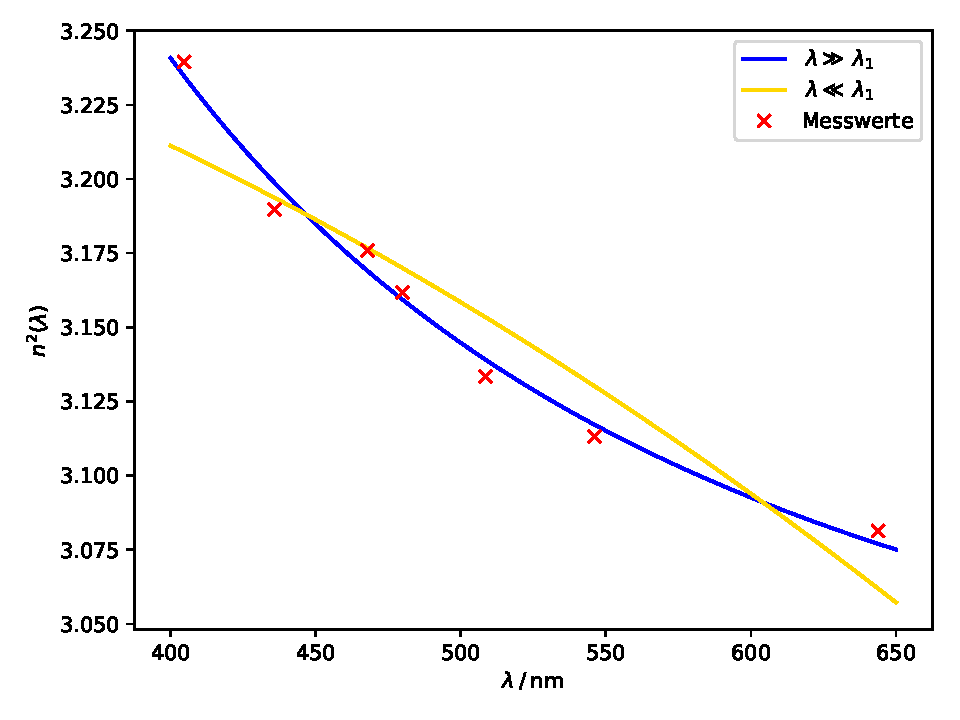
\includegraphics[width=\textwidth]{Plots/n.pdf}
  \caption{$n^2$-$\lambda$-Diagramm zur Bestimmung der Dispersionskurve}
  \label{fig:n}
\end{figure}

Eine Regression $n^2(\lambda) = A_0 + \frac{A_2}{\lambda^2}$ für $\lambda \gg \lambda_1$ ergibt
\begin{align*}
  A_0 &= \SI{2,97(1)}{} \\
  A_2 &= \SI{4,3(7)e4}{\nm \squared}.
\end{align*}

Eine Regression $n^2(\lambda) = A'_0 - A'_2 \lambda^2$ für $\lambda \ll \lambda_1$ ergibt
\begin{align*}
  A'_0 &= \SI{3,31(3)}{} \\
  A'_2 &= \SI{5,9(9)e-7}{\per \nm \squared}.
\end{align*}

Um nun zu bestimmen welche Dispersionskurve die Messwerte besser beschreibt wird die Summe der Abweichungsquadrate berechnet
\begin{align*}
  s^2_\text{n} &= \frac{1}{z-2} \sum_{i=0}^z \left(n^2(\lambda_i) - A_0 - \frac{A_2}{\lambda^2_i} \right)^2 = \SI{4,41e-5}{} \\
  s^2_\text{n'} &= \frac{1}{z-2} \sum_{i=0}^z \left(n^2(\lambda_i) - A'_0 - A'_2 \lambda^2_i \right)^2 = \SI{0,14}{}.
\end{align*}

Daraus ergibt sich, dass die Regression für $\lambda \gg \lambda_1$ die Messwerte am besten beschreibt.
%Diese ist in Abbildung \ref{fig:dis}
%nochmal dargestellt.
%\begin{figure}[H]
%  \centering
%  \includegraphics[width=\textwidth]{Plots/dis.pdf}
%  \caption{$n^2$-$\lambda$-Diagramm mit der gültigen Dispersionskurve}
%  \label{fig:dis}
%\end{figure}

\subsection{Abbe'sche Zahl \label{sec:abbe}}

Die Abbe'sche Zahl ergibt sich aus Gleichung \eqref{eqn:abbe}
\begin{equation}
  \nu = \frac{n_\text{D} - 1}{n_\text{F} - n_\text{C}}.
  \label{eqn:abbe}
\end{equation}

Dabei sind $n_\text{D}$, $n_\text{F}$ und $n_\text{C}$ die Brechungsindizes der Wellenlängen der Frauenhoferschen Linien $\lambda_\text{D} = \SI{589}{\nm}$,
$\lambda_\text{F} = \SI{486}{\nm}$ und $\lambda_\text{C} = \SI{656}{\nm}$.

Nach Kapitel \ref{sec:dis} ergeben sich die Brechungsindizes aus Gleichung \eqref{eqn:ndis}
\begin{equation}
  n(\lambda) = \sqrt{A_0 + \frac{A_2}{\lambda^2}}.
  \label{eqn:ndis}
\end{equation}

Die Fehler berechnen sich aus der Gauß'schen Fehlerfortpflanzung \eqref{eqn:errndis}
\begin{equation}
  \sigma_{n(\lambda)} = \sqrt{\left(\frac{1}{2 \sqrt{A_0 + \frac{A_2}{\lambda^2}}} \sigma_{A_0} \right)^2 + \left( \frac{1}{2 \lambda^2 \sqrt{A_0 + \frac{A_2}{\lambda^2}}} \sigma_{A_2} \right)^2}.
  \label{eqn:errndis}
\end{equation}

Für die Brechungsindizes erhält man
\begin{align*}
  n_\text{D} &= \SI{1,760(3)}{}\\
  n_\text{F} &= \SI{1,753(3)}{}\\
  n_\text{C} &= \SI{1,776(4)}{}.
\end{align*}

Die Abbe'sche Zahl beträgt somit
\begin{equation*}
  \nu = \SI{33(7)}{}.
\end{equation*}

Der Fehler ergibt sich aus Gleichung \eqref{eqn:errabbe}
\begin{equation}
  \sigma_\nu = \sqrt{\left( \frac{1}{n_\text{F}-n_\text{C}} \sigma_{n_\text{D}} \right)^2 + \left(\frac{1-n_\text{D}}{(n_\text{F}-n_\text{C})^2} \sigma_{n_\text{F}} \right)^2 + \left(\frac{n_\text{D}-1}{(n_\text{F}-n_\text{C})^2} \sigma_{n_\text{F}} \right)^2}
  \label{eqn:errabbe}
\end{equation}

Der Theoriewert \cite{sample4} für Schwertflint 14 beträgt $\nu_\text{theo} = \SI{26,5}{}$. Die Abweichung liegt somit bei $\SI{24,12}{\%}$.

\subsection{Auflösungsvermögen}

Das Auflösungsvermögen berechnet sich aus
\begin{equation}
  A = \frac{\lambda}{\symup{\Delta} \lambda} = b \frac{\symup{d} n(\lambda)}{\symup{d} \lambda}.
\end{equation}
\begin{center}
  \tiny{($\lambda \: \hat{=} \: \text{gemittelte Wellenlänge der beiden Spektrallinien}$, $\symup{\Delta}\lambda \: \hat{=} \: \text{Wellenlängenunterschied}$, $b = \SI{3}{\cm} \: \hat{=} \: \text{Basislänge des Prismas}$)}
\end{center}

Für die in Kapitel \ref{sec:dis} bestimmte Dispersionskurve berechnet sich das Auflösungsvermögen aus Gleichung \eqref{eqn:auf} und
dem Fehler \eqref{eqn:errauf}.
\begin{align}
  A &= b \frac{A_2}{\lambda^3 \sqrt{A_0 + \frac{A_2}{\lambda^2}}} \label{eqn:auf} \\
  \sigma_A &= \sqrt{\left(\frac{b A_2}{2 \lambda^3 \left(A_0 + \frac{A_2}{\lambda^2} \right)^{\sfrac{3}{2}}} \sigma_{A_0}\right)^2 + \left(\frac{(2 A_0 \lambda^2) b}{2 \lambda^3 \sqrt{A_0 + \frac{A_2}{\lambda^2}} (A_0 \lambda^2 + A_2)} \sigma_{A_2}\right)^2} \label{eqn:errauf}.
\end{align}

Nach Gleichung \eqref{eqn:auf} und \eqref{eqn:errauf} beträgt das Auflösungsvermögen für die Frauenhoferschen Linien
\begin{align*}
  A_{\lambda_\text{D}} &= \SI{3,6(2)e3}{} \\
  A_{\lambda_\text{F}} &= \SI{2,6(1)e3}{} \\
  A_{\lambda_\text{C}} &= \SI{6,3(3)e3}{}.
\end{align*}

\subsection{Am nächsten gelegene Absorptionsstelle}

Durch einen Koeffizientenvergleich lässt sich die am nächsten gelegene Absorptionsstelle $\lambda_1$ mithilfe von Gleichung \eqref{eqn:l1} berechnen
\begin{equation}
  \lambda_1 = \frac{A_2}{A_0-1}.
  \label{eqn:l1}
\end{equation}

Der Fehler ergibt sich aus \eqref{eqn:errl1}
\begin{equation}
  \sigma_{\lambda_1} = \sqrt{\left(\frac{\left(\frac{A_2}{A_0-1}\right)^{\sfrac{3}{2}}}{2 A_2} \sigma_{A_0}\right)^2 + \left(\frac{\sqrt{\frac{A_2}{A_0-1}}}{2 A_2} \sigma_{A_2} \right)^2} \text{.}
  \label{eqn:errl1}
\end{equation}

Daraus folgt:
\begin{equation*}
  \lambda_1 = \SI{147(4)}{\nm}\text{.}
\end{equation*}
